\begin{figure}[H]
\centering
\begin{tabular}{ccc}
\begin{tabular}{c}

\begin{tikzpicture}[scale=0.7]
    \draw[step=1cm, black, thick] (0,0) grid (4,4);
\end{tikzpicture}
\\
Začetno stanje
\end{tabular}
&
\begin{tabular}{c}
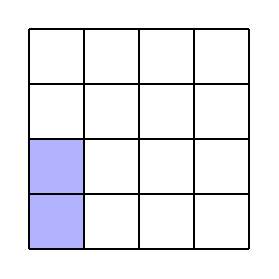
\begin{tikzpicture}[scale=0.7]
    \fill[blue!30] (0,0) rectangle (1,2);
    \draw[step=1cm, black, thick] (0,0) grid (4,4);
\end{tikzpicture}
\\
1. poteza
\end{tabular}
&
\begin{tabular}{c}
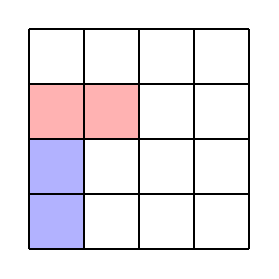
\begin{tikzpicture}[scale=0.7]
    \fill[blue!30] (0,0) rectangle (1,2);
    \fill[red!30] (0,2) rectangle (2,3);
    \draw[step=1cm, black, thick] (0,0) grid (4,4);
\end{tikzpicture}
\\
2. poteza
\end{tabular}
\\[1em]
\begin{tabular}{c}
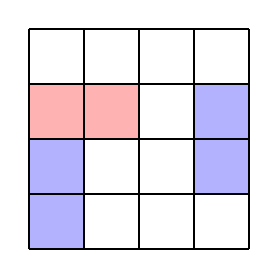
\begin{tikzpicture}[scale=0.7]
    \fill[blue!30] (0,0) rectangle (1,2);
    \fill[red!30] (0,2) rectangle (2,3);
    \fill[blue!30] (3,1) rectangle (4,3);
    \draw[step=1cm, black, thick] (0,0) grid (4,4);
\end{tikzpicture}
\\
3. poteza
\end{tabular}
&
\begin{tabular}{c}
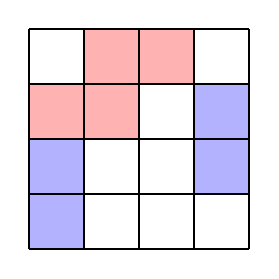
\begin{tikzpicture}[scale=0.7]
    \fill[blue!30] (0,0) rectangle (1,2);
    \fill[red!30] (0,2) rectangle (2,3);
    \fill[blue!30] (3,1) rectangle (4,3);
    \fill[red!30] (1,3) rectangle (3,4);
    \draw[step=1cm, black, thick] (0,0) grid (4,4);
\end{tikzpicture}
\\
4. poteza
\end{tabular}
&
\begin{tabular}{c}
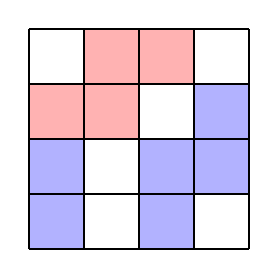
\begin{tikzpicture}[scale=0.7]
    \fill[blue!30] (0,0) rectangle (1,2);
    \fill[red!30] (0,2) rectangle (2,3);
    \fill[blue!30] (3,1) rectangle (4,3);
    \fill[red!30] (1,3) rectangle (3,4);
    \fill[blue!30] (2,0) rectangle (3,2);
    \draw[step=1cm, black, thick] (0,0) grid (4,4);
\end{tikzpicture}
\\
5. poteza
\end{tabular}
\\
\end{tabular}
\caption{Primer poteka igre (zmaga navpični igralec).}
\end{figure}